Microsoft Azure Storage is a cloud storage system that provides customers the ability to store seemingly limitless amounts of data. It has grown from 10s of Petabytes (PB) in 2010 to Exabytes (EB) in 2015, with the total number of objects stored well-exceeding 60 trillion.

Azure Storage vNext is the next generation storage system for Microsoft Azure, where the primary design target is to increase the scalability by more than 100$\times$. Similar to the current system, vNext employs containers, called {\em extents}, to store data. Extents are typically several Gigabytes each, consisting of many data blocks, and replicated over multiple {\em extent nodes} (ENs). However, in contrast to the current system, which employs a Paxos-based, centralized mapping from extents to ENs, vNext achieves its scalability target by employing a completely \emph{distributed mapping}. In vNext, extents are divided into partitions, with each partition managed by a light-weight {\em extent manager} (ExtMgr).

\begin{figure}[t]
\centering
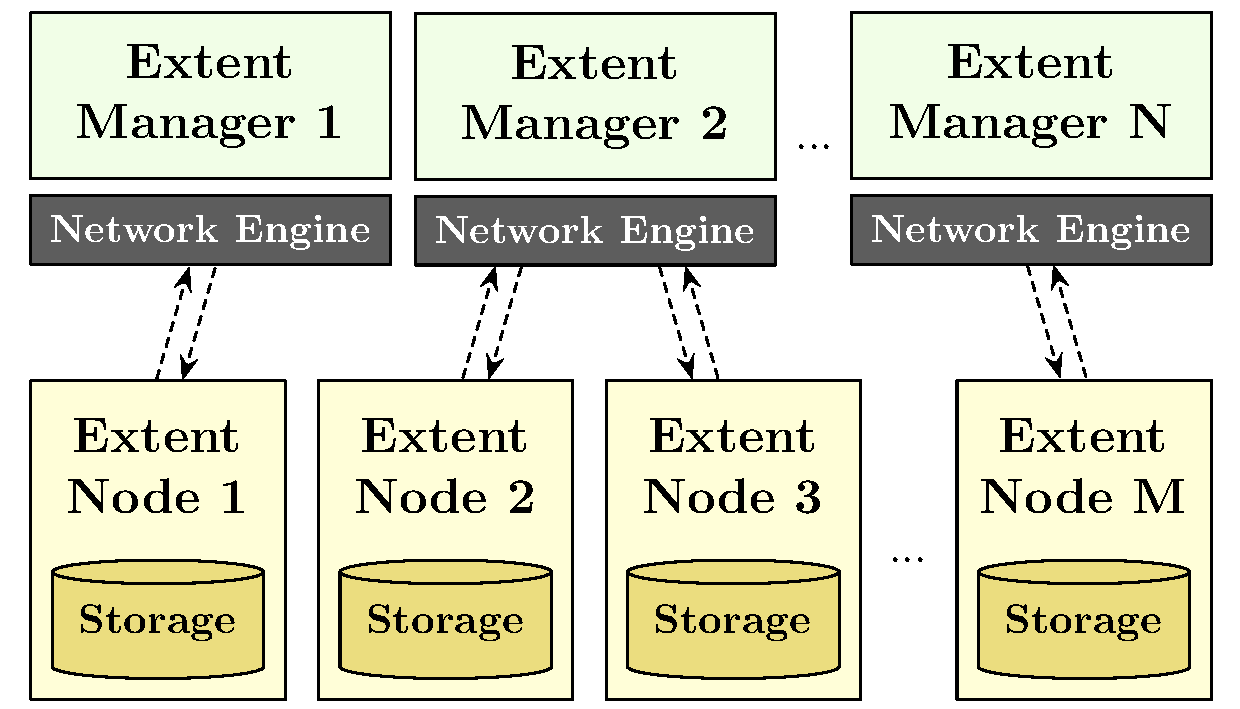
\includegraphics[width=\linewidth]{img/azurestore}
\caption{Top-level components of a distributed extent management system for Windows Azure.}
\label{fig:vnext}
\end{figure}

One of the many responsibilities of an ExtMgr is to ensure that every extent maintains enough \emph{replicas} in the system. To achieve this, an ExtMgr receives frequent periodic \emph{heartbeat} messages from every EN. The failure of an EN is detected by missing heartbeats. An ExtMgr also receives less frequent, but still periodic, {\em synchronization reports} from every EN. The sync reports list all the extents (and associated metadata) stored on the EN. Based on these two types of messages, an ExtMgr identifies which ENs have failed and which extents are affected and missing replicas. The ExtMgr, then, schedules tasks to repair the affected extents and distributes the tasks to ENs. The ENs repair the extents from their existing replicas in the system and lazily update the ExtMgr via future sync reports. All this communication between an ExtMgr and the ENs occurs via network engines installed in each component of vNext (see Figure~\ref{fig:vnext}).

To ensure correctness, the developers of vNext have instrumented extensive, multiple levels of testing:
\begin{enumerate}
\item \emph{Unit testing}, which sends emulated heartbeats and sync reports to an ExtMgr and verifies that the messages are processed as expected.

\item \emph{Integration testing}, which launches an ExtMgr together with multiple ENs, subsequently injects an EN failure, and finally verifies that the affected extents are eventually repaired.

\item \emph{Stress testing}, which launches an ExtMgr with multiple ENs and multiple extents. It keeps repeating the following process: injecting an EN failure, launching a new EN and verifying that the affected extents are eventually repaired.
\end{enumerate}

Despite of the extensive testing efforts, the vNext developers have been plagued by what appears to be an elusive bug in the ExtMgr logic. All the unit test and integration test suites successfully pass every single time. However, the stress test suite fails {\em from time to time} after very long executions, manifested as the replicas of some extents remain missing while never being repaired. The bug appears difficult to identify, reproduce and troubleshoot. First, it takes very long executions to trigger. Second, an extent not being repaired is {\em not} a property that can be easily verified. In practice, the developers rely on very large time-out period to detect the bug. Finally, by the time that the bug is detected, very long execution traces have been collected, which makes manual inspection tedious and ineffective.

To uncover this bug and many other similar ones, the developers are in constant search of a generic and systematic approach for testing distributed storage systems.

%Since this is a rather typical dilemma in the development of distributed storage systems, a general and systematic approach hopefully would be very helpful to the developers and greatly increase their productivity.
